\documentclass[a4paper,11pt]{article}
\usepackage{amsmath,amsthm,amsfonts,amssymb,amscd,amstext,vmargin,graphics,graphicx,tabularx,multicol} 
\usepackage[francais]{babel}
\usepackage[utf8]{inputenc}  
\usepackage[T1]{fontenc} 
\usepackage{pstricks-add,tikz,tkz-tab,variations}
\usepackage[autolanguage,np]{numprint} 

\setmarginsrb{1.5cm}{0.5cm}{1cm}{0.5cm}{0cm}{0cm}{0cm}{0cm} %Gauche, haut, droite, haut
\newcounter{numexo}
\newcommand{\exo}[1]{\stepcounter{numexo}\noindent{\bf Exercice~\thenumexo} : \marginpar{\hfill /#1}}
\reversemarginpar


\newcounter{enumtabi}
\newcounter{enumtaba}
\newcommand{\q}{\stepcounter{enumtabi} \theenumtabi.  }
\newcommand{\qa}{\stepcounter{enumtaba} (\alph{enumtaba}) }
\newcommand{\initq}{\setcounter{enumtabi}{0}}
\newcommand{\initqa}{\setcounter{enumtaba}{0}}

\newcommand{\be}{\begin{enumerate}}
\newcommand{\ee}{\end{enumerate}}
\newcommand{\bi}{\begin{itemize}}
\newcommand{\ei}{\end{itemize}}
\newcommand{\bp}{\begin{pspicture*}}
\newcommand{\ep}{\end{pspicture*}}
\newcommand{\bt}{\begin{tabular}}
\newcommand{\et}{\end{tabular}}
\renewcommand{\tabularxcolumn}[1]{>{\centering}m{#1}} %(colonne m{} centrée, au lieu de p par défault) 
\newcommand{\tnl}{\tabularnewline}

\newcommand{\bmul}[1]{\begin{multicols}{#1}}
\newcommand{\emul}{\end{multicols}}

\newcommand{\trait}{\noindent \rule{\linewidth}{0.2mm}}
\newcommand{\hs}[1]{\hspace{#1}}
\newcommand{\vs}[1]{\vspace{#1}}

\newcommand{\N}{\mathbb{N}}
\newcommand{\Z}{\mathbb{Z}}
\newcommand{\R}{\mathbb{R}}
\newcommand{\C}{\mathbb{C}}
\newcommand{\Dcal}{\mathcal{D}}
\newcommand{\Ccal}{\mathcal{C}}
\newcommand{\mc}{\mathcal}

\newcommand{\vect}[1]{\overrightarrow{#1}}
\newcommand{\ds}{\displaystyle}
\newcommand{\eq}{\quad \Leftrightarrow \quad}
\newcommand{\vecti}{\vec{\imath}}
\newcommand{\vectj}{\vec{\jmath}}
\newcommand{\Oij}{(O;\vec{\imath}, \vec{\jmath})}
\newcommand{\OIJ}{(O;I,J)}


\newcommand{\reponse}[1][1]{%
\multido{}{#1}{\makebox[\linewidth]{\rule[0pt]{0pt}{20pt}\dotfill}
}}

\newcommand{\titre}[5] 
% #1: titre #2: haut gauche #3: bas gauche #4: haut droite #5: bas droite
{
\noindent #2 \hfill #4 \\
#3 \hfill #5

\vspace{-1.6cm}

\begin{center}\rule{6cm}{0.5mm}\end{center}
\vspace{0.2cm}
\begin{center}{\large{\textbf{#1}}}\end{center}
\begin{center}\rule{6cm}{0.5mm}\end{center}
}



\begin{document}
\pagestyle{empty}
\titre{Interrogation: Les statistiques}{Nom :}{Prénom :}{Classe}{Date}

\vspace*{0.2cm}

\begin{flushleft}
\begin{tabular}{|m{9.5cm}|m{1.25cm}|m{1.25cm}|m{1.25cm}|m{1.25cm}|m{1.25cm}|}
\hline 
\textbf{Compétences} & \begin{center}
\textbf{N.E.}
\end{center} & \begin{center}
\textbf{M.I.}
\end{center} & \begin{center}
\textbf{M.F.}
\end{center}  & \begin{center}
\textbf{M.S.}
\end{center} & \begin{center}
\textbf{T.B.M.}
\end{center} \\ 
\hline 
Je dois savoir calculer des effectifs, des fréquences, moyennes (liste, tableau, graphique, tableur) &  &  & & &\\
\hline 
Je dois savoir lire et interpréter des données sous forme de données brutes, de tableau, de diagramme (diagramme en bâtons, diagramme circulaire, histogramme) &  &  & & &\\
\hline

\end{tabular} 
\end{flushleft}

\textit{N.E = Non évalué ; M.I. = Maîtrise insuffisante ; M.F. = Maîtrise fragile ; M.S. = Maîtrise satisfaisante ; T.B.M. = Très bonne maîtrise}\\

\vspace*{0.5cm}
\exo{3} 
La course automobile des 24 heures du Mans consiste à effectuer en 24 heures le plus grand nombre de tours d'un circuit.\\
Le diagramme en bâtons ci-dessous donne la répartition du nombre de tours effectués par les coureurs automobiles en tête du rallye.

\bmul{2}

\includegraphics[scale=1]{histo1.eps} 

\columnbreak

\q Quels sont les valeurs extrêmes de cette série ?\\
\reponse[2]\\

\q Quel est effectif total de cette série ?\\
\reponse[3]\\


\emul

\q Quel est le pourcentage de coureurs ayant effectués plus de 330 tours de circuit ?\\
\reponse[3]\\

\q Calculer la moyenne de cette série (on donnera la valeur arrondie à l'unité)\\
\reponse[5]\\

\newpage
\vspace*{0.3cm}

\exo{4} 
Les résultats chronométrés de l'épreuve du 60 m pour les garçons de 14 ans du collège ont été regroupés dans le tableau suivant :

\renewcommand{\arraystretch}{1.5}

\begin{flushleft}
\begin{tabular}{|m{3cm}|c|c|c|c|c|}
\hline 
\textbf{Temps t} (en s) & $8,4 \leq t < 8,9$ & $8,9 \leq t < 9,4$ & $9,4 \leq t < 9,9$& $9,9 \leq t < 10,4$ & $10,4 \leq t < 10,9$ \\ 
\hline 
\textbf{Nombre d'élèves} & 3 & 9 & 15 & 6 & 4\\ 
\hline 
\textbf{Effectifs cumulés croissants} &  &  &  &  &  \\ 
\hline 
\textbf{Fréquences} (en $\%$) &  &  &  &  &  \\ 
\hline 
\end{tabular} 
\end{flushleft}

\initq 

\q Compléter le tableau ci-dessus. Les fréquences seront données en pourcentage arrondies au dixième près.\\

\q   Quel est  le  pourcentage  d'élèves  ayant  couru le 60 m en moins de 9,4 secondes ?\\
\reponse[2]\\

\q Quelle est la performance moyenne d'un garçon de 14 ans, sur 60 m, dans ce collège ?\\
\reponse[4]\\

\vspace*{0.2cm}

\exo{3}
Un industriel a commandé un lot de 100 pièces dont le diamètre doit mesurer 55 mm.\\
Il est convenu qu'à la réception du lot, il fera une vérification et n'acceptera la livraison que si les deux conditions suivantes sont réalisées simultanément :\\

\bi
\item \underline{Condition 1 }: L'écart entre le diamètre voulu (55 mm) et la moyenne  M  des mesures faites sur le lot est inférieur à 0,04 mm.\\

\item \underline{Condition 2 }: Au moins 60 $\%$ des pièces du lot ont un diamètre \textit{d} appartenant à l'intervalle $]54,94 ; 55,06[$.\\

\ei

Les mesures faites sur le lot ont donné la série statistique suivante :\\

\begin{tabular}{|m{3cm}|c|c|c|c|c|c|c|c|c|c|c|}
\hline 
\textbf{Mesures en mm des diamètres \textit{d} }& 54,75 & 54,80 & 54,85 & 54,90 & 54,95 & 55 & 55,05 & 55,10 & 55,15 & 55,20 & 55,25 \\ 
\hline 
\textbf{Effectifs} & 4 & 5 & 7 & 11 & 12 & 36 & 19 & 3 & 2 & 1 & 0  \\ 
\hline 
\end{tabular} 

\vspace*{0.3cm}

$\rightarrow$ Le lot est-il accepté ou refusé ? \textbf{Justifier la réponse}.\\
\reponse[8]\\



\end{document}
